\section{Resultados}

Tras la obtención de la red de genes al realizar el mapeo con STRINGdb hemos obtenido un grafo como el que podemos observar en la figura \ref{fig:graph1}. En este grafo podemos observar todos los genes que pertenecen a la red asociada al fénomeno de Raynaud. Esto se ha obtenido a partir de STRINGdb como hemos explicado en el apartado \ref{obtencion_ref}.

\begin{minipage}{\linewidth}
	\makebox[\linewidth]{
		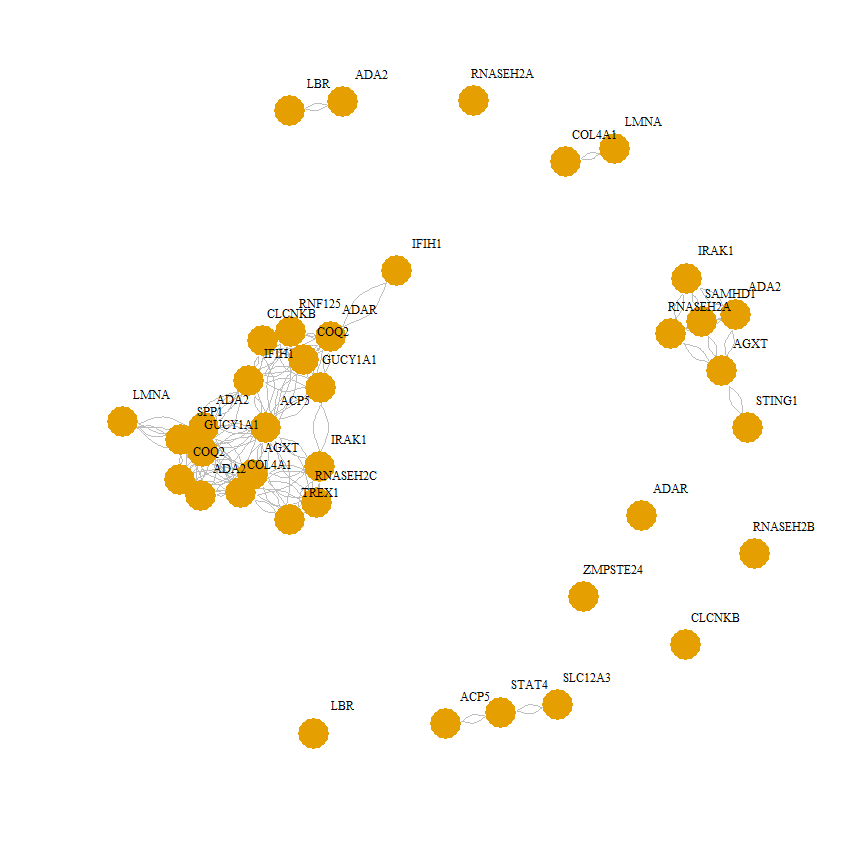
\includegraphics[width=\textwidth]{figures/Raynaud_genes-graph.png}
	}
	\captionof{figure}{Grafo obtenido al realizar el mapeo de genes}
	\label{fig:graph1}
\end{minipage}

Seguidamente hemos obtenido las comunidades que conforman nuestra red y a las que posteriormente se le harán los estudios de funcionalidad y podremos comprobar que genes conforman el fenotipo más grave de la enfermedad. Se han obtenido 3 gráficas en las que mostramos información acerca de estas comunidades.

En la figura \ref{fig:dendrogram}, la primera obtenida del flujo de trabajo, se observa un dendrograma en la que, diferenciadas por colores, se pueden visualizar las diferentes comunidades obtenidas. Estas se han obtenido a una altura bastante alta (alrededor del 0.9) y nos indica que tenemos 6 comunidades cuyo agrupamiento más grande tiene 11 genes.

\begin{minipage}{\linewidth}
	\makebox[\linewidth]{
		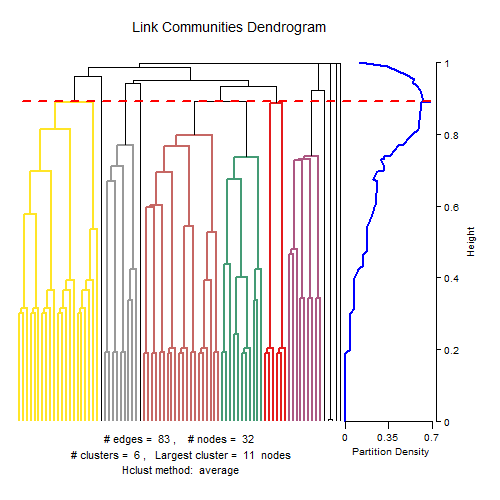
\includegraphics[width=0.8\textwidth]{figures/Raynaud_genes-dendrogram.png}
	}
	\captionof{figure}{Dendrograma de la red mostrando las comunidades}
	\label{fig:dendrogram}
\end{minipage}

La segunda figura que obtenemos del flujo de trabajo sería la número \ref{fig:members}, en esta observamos una matriz de los miembros de cada comunidad. En este caso solo podemos ver los 10 primeros genes de nuestra red y en la matriz se nos muestra las comunidades a las que pertenece cada gen (señalado con un cuadrado en color para cada comunidad a la que pertenece). Además en los márgenes derecho e inferior de la matriz observamos los sumatorios del número de total de comunidades a las que pertenece cada gen y el número de genes que contiene cada comunidad, respectivamente.

\begin{minipage}{\linewidth}
	\makebox[\linewidth]{
		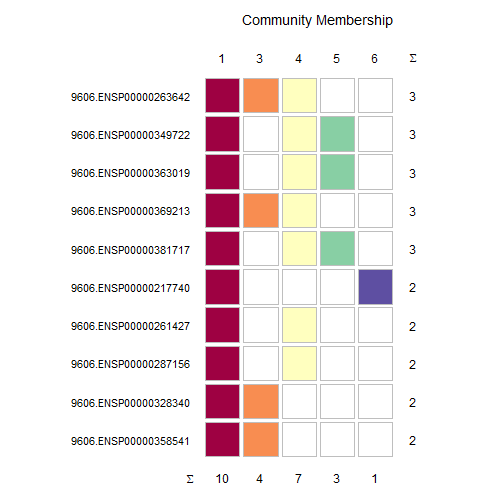
\includegraphics[width=0.8\textwidth]{figures/Raynaud_genes-comunity_members_matrix.png}
	}
	\captionof{figure}{Matriz de los primeros genes para cada comunidad}
	\label{fig:members}
\end{minipage}

Por último, al obtener las comunidades también hemos mostrado la figura \ref{fig:comunity_graph} en la que se observa un grafo similar al de la figura \ref{fig:graph1}, sin embargo, en este tenemos diferenciadas por colores las diferentes comunidades que hemos obtenido tras realizar el flujo de trabajo.

\begin{minipage}{\linewidth}
	\makebox[\linewidth]{
		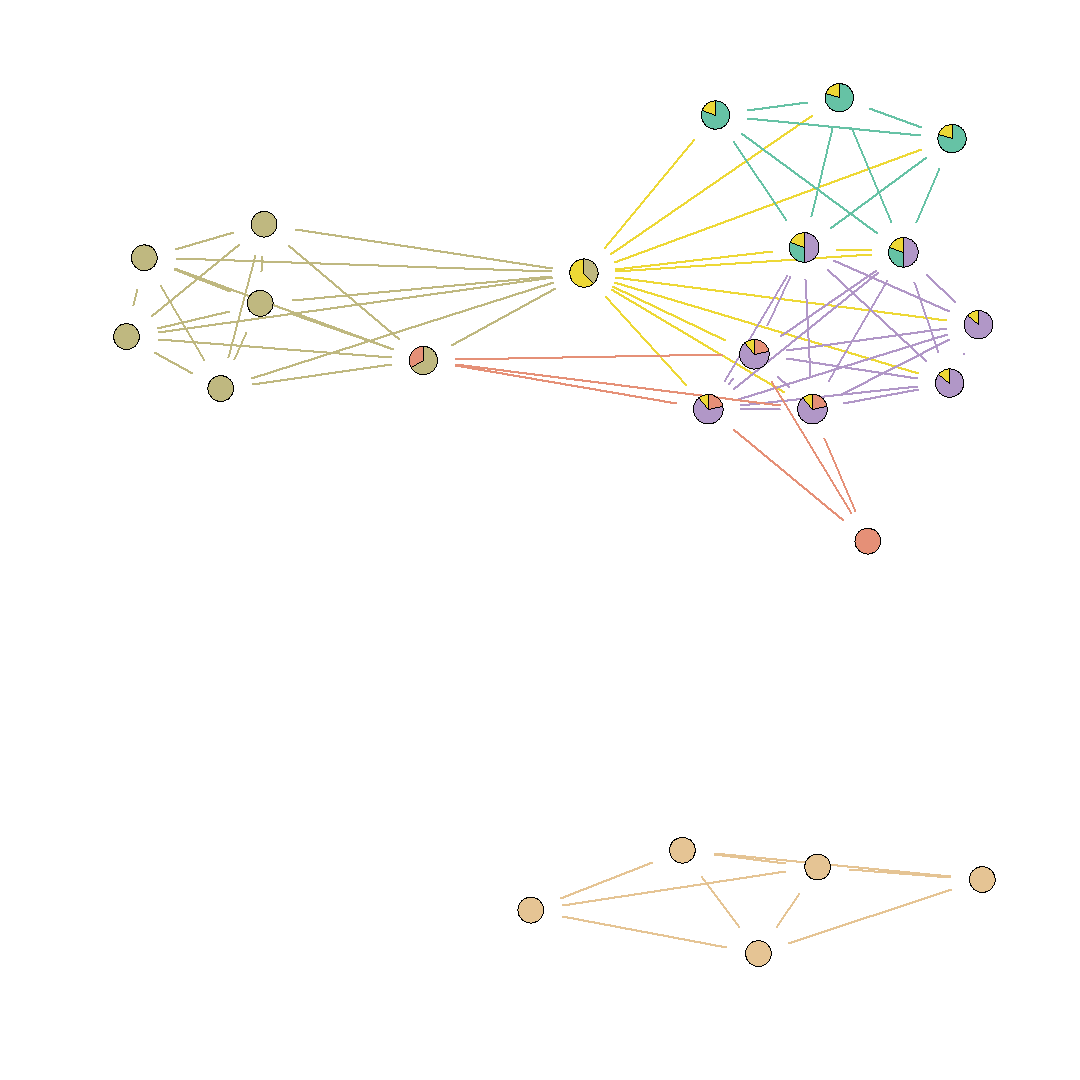
\includegraphics[width=0.8\textwidth]{figures/Raynaud_genes-comunities_graph.png}
	}
	\captionof{figure}{Grafo de los genes divididos por comunidad}
	\label{fig:comunity_graph}
\end{minipage}
